% !TEX root = ../Projektdokumentation.tex
\section{Beispiel 1}
\label{sec:beispiel1}


\subsection{Ausgangssituation} 
\label{sec:ausgangssituation1}
Im ersten Beispiel wird eine Wahl untersucht, in der jeder Teilnehmer alle Kandidaten bewertet hat und damit eine eindeutige Reihenfolge der Kandidaten generiert werden kann. Kein Kandidat wurde gleichbehandelt oder nicht bewertet.

Bildhaft wird die \schulze in folgender Ausgangssituation eingesetzt:
Ein Kurs von 28 Studierenden wählt einen Kurssprecher. Zur Wahl stellt sich Anton (Kandidat $a$), Berta (Kandidatin $b$), Conny (Kandidatin $c$) und Dennis (Kandidat $d$).

Jeder der 28 Studierenden muss die Kandidaten nach Erst-, Zweit-, Dritt- und Viertwunsch ordnen. Nach der Auszählung hat sich Folgende Situation eingespielt. 

\begin{description}
\centering
\item[6 mal] $a \succ_{v} b \succ_{v} d \succ_{v}c$
\item[4 mal] $c \succ_{v} a \succ_{v} b \succ_{v}d$
\item[10 mal] $b \succ_{v} d \succ_{v} a \succ_{v}c$
\item[3 mal] $b \succ_{v} a \succ_{v} d \succ_{v}c$
\item[5 mal] $d \succ_{v} c \succ_{v} b \succ_{v}a$
\end{description}

Dies bedeutet beispielhaft für die erste Zeile, dass sechs Mal Wahlzettel abgegeben wurden, die Anton als Erstwunsch, Berta als Zweitwunsch, Dennis als Drittwunsch und Conny als Viertwunsch angegeben haben.

Diese Auszählung der Wahl wird nun in die \schulze überführt und bewertet.
\newpage
\subsection{Lösungsschritte} 
\label{sec:loesungen1}
Um die \schulze anzuwenden, muss zuerst die Menge $N$ bestimmt werde. Diese Menge bildet sich, indem jeder Kandidat gegen jeden Kandidaten antritt.

Exemplarisch wird das Duell $a$ gegen $b$ durchgeführt und die Kandidaten $c$ und $d$ ignoriert. Es können diese Kandidaten im Duell ignoriert werden, da es irrelevant ist, wo das Duell stattfindet, ob die beiden Kandidaten Dritt- und Viertwunsch sind oder ein Kandidat Erstwunsch und der andere Zweitwunsch ist. Die Betrachtung der genauen Platzierungen ergibt sich durch die Betrachtung aller Kandidaten mit diesem Verfahren.

\begin{description}
\centering
\item[6 mal] $a \succ_{v} b$
\item[4 mal] $a \succ_{v} b$
\item[10 mal] $b \succ_{v} a$
\item[3 mal] $b \succ_{v} a$
\item[5 mal] $b \succ_{v}a$
\end{description}

Wird nun dieses Duell betrachte, erhalten Kandidat $a$ 10 Stimmen und Kandidat $b$ 18 Stimmen und Kandidat $b$ gewinnt damit.


Wenn dies für alle Duelle gemacht wurde, ergibt sich folgendes Ergebnis.
 \begin{description}
 \centering
 \item[$a$ vs. $b$] 10 Stimmen gegen 18 Stimmen, $b$ gewinnt
 \item[$a$ vs. $c$] 19 Stimmen gegen 9 Stimmen, $a$ gewinnt
 \item[$a$ vs. $d$] 13 Stimmen gegen 15 Stimmen, $d$ gewinnt
 \item[$b$ vs. $c$] 19 Stimmen gegen 9 Stimmen, $b$ gewinnt
 \item[$b$ vs. $d$] 23 Stimmen gegen 5 Stimmen, $b$ gewinnt
 \item[$c$ vs. $d$] 4 Stimmen gegen 24 Stimmen, $d$ gewinnt
 \end{description}
 
 Mit diesen Werten kann man nun die Menge $N$, wie sie in Tabelle \ref{Beispie1_N} zu sehen ist, aufstellen.

% !TEX root = Projektdokumentation.tex
\begin{longtable}[c]{|l|l|l|l|l|}
\hline
            & N{[}*,a{]} & N{[}*,b{]} & N{[}*,c{]} & N{[}*,d{]} \\ \hline
\endfirsthead
%
\endhead
%
N{[}a, *{]} & ---        & 10         & 19         & 13         \\ \hline
N{[}b, *{]} & 18         & ---        & 19         & 23         \\ \hline
N{[}c, *{]} & 9          & 9          & ---        & 4          \\ \hline
N{[}d, *{]} & 15         & 5          & 24         & ---        \\ \hline
\caption{Die Menge $N$ in Beispiel 1}
\label{Beispie1_N}\\
\end{longtable}

Im nächsten Schritt müssen die Wege zwischen den Kandidaten gesucht werden, wie es in der Definition in Abschnitt \ref{itm:def231} unter (2.3.1) beschreiben wird. Zyklische Verbindungen sind nicht erlaubt.

In Abbildung \ref{fig:graph1} ist die Menge $N$ als gerichteter Graph aufgezeichnet.

\begin{figure}[!h]
\centering
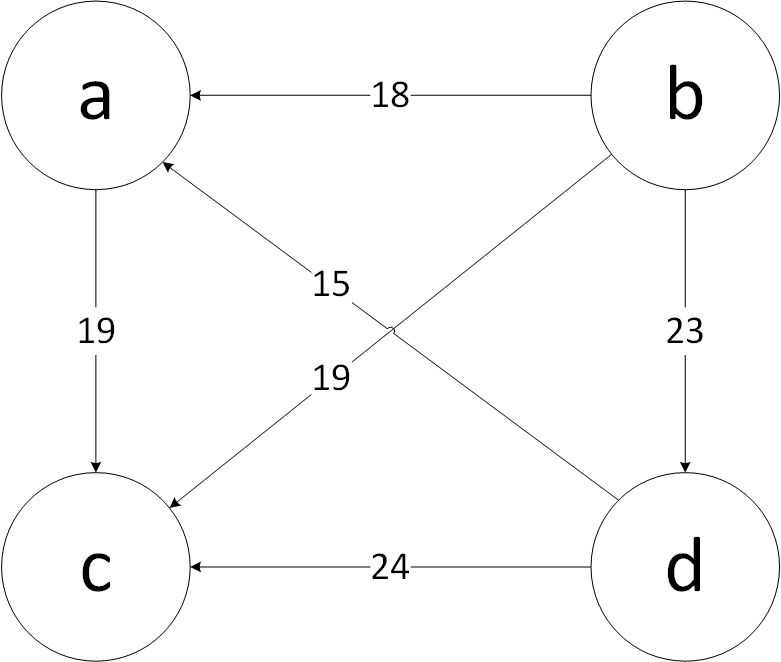
\includegraphics[scale=0.5]{Bilder/Beispiel1_Graph.png}
\caption{Graph über die Menge $N$ (Beispiel 1)}
\label{fig:graph1}
\end{figure}

In dem Graphen wurden gerichtete Kanten vom Sieger in die Richtung des Verlierers gezogen und das Kantengewicht des Siegers der Duelle aufgetragen. Dies sind die unter Abschnitt \ref{verbindung} beschriebenen Verbindungen. Nun muss aus der Definition in Abschnitt \ref{itm:def233} (2.3.2) und  (2.3.3) angewendet werden, um die Menge $P$ zu bilden, die die Stärksten Wege beinhaltet.

Dazu werden nun alle Wege zwischen den Kandidaten gebildet und der stärkste Weg, das ist jener, bei dem die schwächste Verbindung am größten ist, ausgewählt für die Menge $P$.

\begin{description}
\item[$a \to b$:] Es gibt keinen Weg, der von $a$ nach $b$ führt.

\item[$b \to a$:] Es gibt zwei Wege, die von $b$ nach $a$ führen.
	\begin{description}
	\item[Weg 1:] $b$, 23, $d$, 15, $a$, der die Stärke $min_{D}\{23, 15 \}\approx_{D}15$ hat.
	\item[Weg 2:] $b$, 18, $a$, der die Stärke 18 hat.
	\end{description}
	Damit ist ergibt sich die Stärke des stärksten Weges mit Hilfe von $max_{D}\{15, 18\}\approx_{D}18$
	
\item[$a \to c$] Es gibt einen Weg, der von $a$ nach $c$ führt.
	\begin{description}
	\item[Weg 1:] $a$, 19, $c$, der die Stärke 19 hat.
	\end{description}
	Damit ist die Stärke des stärksten Weges auch 19.
	
\item[$c \to a$] Es gibt keinen Weg, der von $c$ nach $a$ führt.

\item[$a \to d$] Es gibt keinen Weg, der von $a$ nach $d$ führt.

\item[$d \to a$] Es gibt einen Weg, der von $d$ nach $a$ führt.
	\begin{description}
	\item[Weg 1:] $d$, 15, $a$, der die Stärke 15 hat.
	\end{description}
	Damit ist die Stärke des stärksten Weges auch 15.
	
\item[$b \to c$:] Es gibt drei Wege, die von $b$ nach $c$ führen.
	\begin{description}
	\item[Weg 1:] $b$, 18, $a$, 19, $c$, der die Stärke $min_{D}\{18, 19 \}\approx_{D}18$ hat.
	\item[Weg 2:] $b$, 19, $c$, der die Stärke 19 hat.
	\item[Weg 3:] $b$, 23, $d$, 24, $c$, der die Stärke $min_{D}\{23, 24 \}\approx_{D}23$ hat.
	\end{description}
	Damit ist ergibt sich die Stärke des stärksten Weges mit Hilfe von $max_{D}\{18, 19, 23 \}\approx_{D}23$
	
\item[$c \to b$] Es gibt keinen Weg, der von $c$ nach $b$ führt.

\item[$b \to d$] Es gibt einen Weg, der von $b$ nach $d$ führt.
	\begin{description}
	\item[Weg 1:] $b$, 23, $d$, der die Stärke 23 hat.
	\end{description}
	Damit ist die Stärke des stärksten Weges auch 23.
	
\item[$d \to b$] Es gibt keinen Weg, der von $d$ nach $b$ führt.

\item[$c \to d$] Es gibt keinen Weg, der von $c$ nach $d$ führt.
	
\item[$d \to c$] Es gibt einen Weg, der von $d$ nach $c$ führt.
	\begin{description}
	\item[Weg 1:] $d$, 24, $c$, der die Stärke 24 hat.
	\end{description}
	Damit ist die Stärke des stärksten Weges auch 24.	
\end{description}

So wurden alle Wege bestimmt und die kritischen Verbindungen gefunden, sodass sich in Tabelle \ref{beispiel1p} die Menge $P$ bildet.

% !TEX root = ../Projektdokumentation.tex

\begin{longtable}[c]{|l|l|l|l|l|}
\hline
             & P{[}*,a{]} & P{[}*,b{]} & P{[}*,c{]} & P{[}*,d{]} \\ \hline
\endfirsthead
%
\endhead
%
P{[}a, *{]} & ---        & ---        & 19         & ---        \\ \hline
P{[}b, *{]} & 18         & ---        & 23         & 23         \\ \hline
P{[}c, *{]}  & ---        & ---         & ---        & ---         \\ \hline
P{[}d, *{]}  & 15         & ---         & 24         & ---        \\ \hline
\caption{Die Menge $P$ (Beispiel 1)}
\label{beispiel1p}\\
\end{longtable}

Die Simulation der Duelle wird für die Kandidaten erneut gemacht, dieses Mal jedoch über die Menge $P$. Wenn es keinen Weg zwischen den Kandidaten gibt, also in der Tabelle ein '---' steht, so wird diese Verbindung als eine Verbindung mit der Stärke 0 betrachtet.

Dieses Ergebnis wird in der Relation $\mathcal{O}$, wie in der Definition (2.3.4) in Abschnitt \ref{itm:def234} beschreiben.
\newpage
\begin{description}
\item[$a$ gewinnt gegen $b$]: nein, daher kein Teil von $\mathcal{O}$ 
\item[$a$ gewinnt gegen $c$]: ja, daher Teil von $\mathcal{O}$ 
\item[$a$ gewinnt gegen $d$]: nein, daher kein Teil von $\mathcal{O}$ 
\item[$b$ gewinnt gegen $a$]: ja, daher Teil von $\mathcal{O}$ 
\item[$b$ gewinnt gegen $c$]: ja, daher Teil von $\mathcal{O}$ 
\item[$b$ gewinnt gegen $d$]: ja, daher Teil von $\mathcal{O}$ 
\item[$c$ gewinnt gegen $a$]: nein, daher nicht Teil von $\mathcal{O}$ 
\item[$c$ gewinnt gegen $b$]: nein, daher nicht Teil von $\mathcal{O}$ 
\item[$c$ gewinnt gegen $d$]: nein, daher nicht Teil von $\mathcal{O}$ 
\item[$d$ gewinnt gegen $a$]: ja, daher Teil von $\mathcal{O}$ 
\item[$d$ gewinnt gegen $b$]: nein, daher nicht Teil von $\mathcal{O}$ 
\item[$d$ gewinnt gegen $c$]: ja, daher Teil von $\mathcal{O}$ 
\end{description} 

Daher ergibt sich $\mathcal{O} = \{ ac,ba,bc,bd,da,dc \}$

\subsection{Ergebnis} 
\label{sec:ergebnis1}
Um den Sieger aus der Relation $\mathcal{O}$ zu finden muss, wie in der Definition in Abschnitt \ref{itm:def235} Punkt (2.3.5) beschreiben, sichergestellt werden, dass ein Sieger nur ein Kandidat sein kann, der im direkten Duell nie durch einen anderen Gegner geschlagen wird.

Um das zu prüfen, wird die Relation $\mathcal{O}$ durchgegangen und geprüft, ob es einen Kandidaten gibt, der immer nur auf der linken Seite eine Tupel z.B: ''bd'' steht und damit immer der Gewinner ist und nie geschlagen wurde, dann würde er auf der rechten Seite des Tupels stehen.

Für dieses Beispiel ergibt sich, dass es nur einen Sieger in der Menge $\mathcal{S}=\{b\}$ gibt, den Kandidaten $b$. Damit wurde mit der \schulze festgestellt, dass Kandidatin Berta die Wahl gewonnen hat.

Zu Beginn des Beispiels konnte man sehen, dass Kandidatin Berta beim Duell mit den anderen Kandidaten gegen alle anderen Kandidaten gewonnen hat. Und es stellt sich daher die Frage, wieso nicht an dieser Stelle schon die Siegerin festgelegt wurde? Dieses Beispiel hat gezeigt, dass die \schulze das \condorcet Kriterium \ref{sec:condorectKriterium} erfüllt, das besagt, dass ein Kandidat, der gegen alle Gegner gewonnen hat auch der Sieger der Wahlmethode, hier der \schulze sein muss. Das Beispiel 2 in Abschnitt \ref{sec:beispiel2} zeigt, dass auch wenn kein \condorcetSieger existiert, ein Sieger mit der Schulze Methode ermittelt werden kann.



